\documentclass[main.tex]{subfiles}
\begin{document}
\newpage
\section{Telegrafenrauschen in Samarium-Erbium-Ferrit}
\todo{ Samarium-Erbium-Ferrit oder Samarium-Erbium-Orthoferrit (oder einfach Verhältnisformel)}
\todo{Roter Faden!}
\todo{Überschriften}
\todo{in plots Variable Kursiv und Variable statt englischer Beschreibung}
\todo{\(B_c\) statt \(B_z\)}
\todo{\(m_c\) statt \(\mu_c\)}
\todo{Grid bei Logaritmischen plots}
\todo{gibt es offizielle namen für die verwendeten Eigenbezeichnungen?}

\todo{Autocovarianz mit log y-Achsen plotten}
\todo{Autokorrelation und Autocovarianz konsistent halten}
Der Orthoferrit besteht aus vier Untergittern, welche jeweils eine andere Magnetisierung \(\vec{\mu}_i\) besitzen (Normiert \(\vec{S}_i\)). Im nachfolgenden Bereich wird die normierte resultierende Magnetisierung (Überlagerung der vier Untergitter) verwendet.

\begin{align}
    \mu_{1} &=  \mu_{2} = \mu_{3} = \mu_{4} = \num{3.66}\mu_B \\
    \vec{m} &= \frac{1}{4} \sum_{i=1}^4 \vec{S}_i
\end{align}

Das Telegrafenrauschen tritt am untersuchten Reorientierungsübergang in c-Richtung auf, weshalb nur diese Komponente betrachtet wird. 

\todo{plot Reorientierungsübergang?}

Eine Simulation, von einem \(128 \times 128 \times 128\) Gitter mit einem simulierten Zeitraum von \SI{1.2}{\nano\second} mit einer numerischen Schrittweite von \SI{20}{\femto\second} benötigt etwa drei Tage Rechenzeit auf einer Nvidea RTX 2080 Ti Grafikkarte. 

In diesem Simulationszeitraum sind im optimalen Temperaturbereich (um mehrere eindeutige Schaltvorgänge zu beobachten) etwa 15-25 Schaltvorgänge pro Simulation zu beobachten vgl. \cref{fig:bsp-run}

Um mehr Schaltvorgänge pro Simulation betrachten zu können, wurde der Simulationszeitraum teilweise verdoppelt.

\begin{figure}[h]
    \centering
    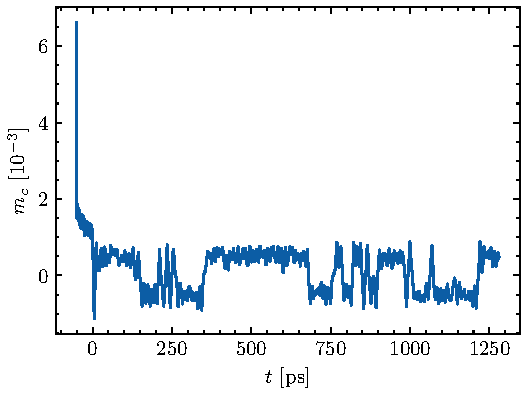
\includegraphics{bilder/plots/theo-vis/example-telegraph-sim.pdf}
    \caption{Einzelne Simulationskurve von \(m_c\) bei \(T \approx \SI{302}{\kelvin}\). Im Zeitraum \(<0\) ist hierbei der Einschwingvorgang zu sehen \todo{Bezeichnung für die zwei Niveaus/Zustände?}
    }\label{fig:bsp-run}
\end{figure}

Die mittleren Aufenthaltszeiten (MDT) in den beiden Niveaus befinden sich in der gleichen Größenordnung, wie der Simulationszeitraum. Um auch bei weniger optimalen Daten, wie in \cref{fig:extraktion-tgr}, eine gute Extraktion des Telegrafenrauschens zu ermöglichen, wurden teilweise die Signale mehrerer Simulationsläufe hintereinander gehängt, um ein langes Signal zu erhalten.

Da aber nicht Zufälligerweise alle Simulationsläufe immer im gleichen Niveau starten und aufhören (so lange die Wahrscheinlichkeit für einen Zustand nicht deutlich höher ist), werden hierbei teilweise zusätzliche Schaltvorgänge hinzugefügt.

\todo{warum ist das meißtens kein problem?}

Andere Möglichkeiten um die Rechenzeit zu verringern wären zum Beispiel eine geringere Gittergröße, oder eine größere Zeitschrittweite.

Die Gittergröße ist allerdings bereits recht klein und eine größere Zeitschrittweite würde die Genauigkeit der Simulation verringern, sodass die Ergebnisse nicht mehr mit den experimentellen Daten vergleichbar wären. Bei einer Schrittweite von \SI{100}{\femto\second} (wahrscheinlich aber schon früher) tritt das Telegrafenrauschen garnicht mehr auf und der Betrag der Magnetisierung ist deutlich größer.

\todo{was passiert im Einschwingvorgang?}

\subsection{Extraktion des Telegrafenrauschens}

\begin{figure}[H]
    \centering
    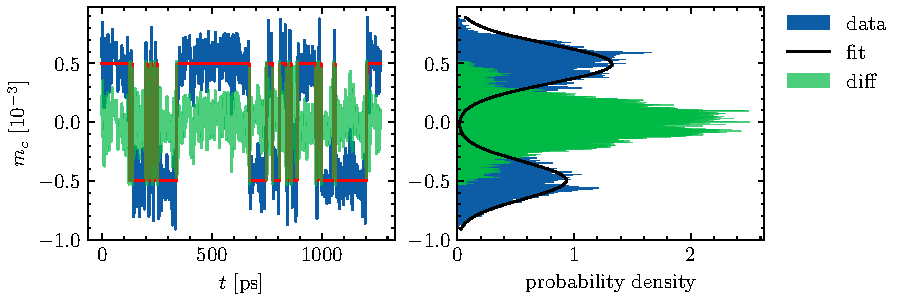
\includegraphics{bilder/plots/Bz_0mT/mc_fit_hist_part2_26.03meV.pdf}
    \caption{Extraktion des Telegrafenrauschen mithilfe des Algorithmus aus \cref{algo}. Das bereinigte Telegrafenrauschen ist im linken Plot in rot zu sehen. Die Differenz zwischen bereinigtem Telegrafenrauschen und dem rohen Signal ist in grün zu sehen.}\label{fig:extraktion-tgr}
\end{figure}

Die Aufenthaltswahrscheinlichkeit zwischen den zwei Zuständen ist deutlich größer, als bei zwei überlagerte Gaußverteilungen anzunehmen wäre. Bei Zwei Lorenzverteilungen ist die Aufenthaltswahrscheinlichkeit im Randbereich jedoch gar nicht passend.

\begin{figure}[H]
    \centering
    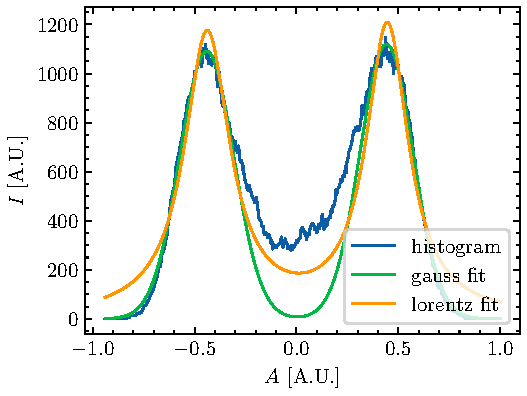
\includegraphics{bilder/plots/theo-vis/hist_fit_comp.pdf}
    \caption{Vergleich von verschiedenen Verteilungsfunktionen um die Wahrscheinlichkeitsdichte zu fitten}\label{fig:fit_func_comp}
\end{figure}

Theoretisch existiert auch noch ein dritter, weniger stabiler, Zustand, der Genau Zwischen den Zwei Niveaus liegt. Dieser sorgt für die Abweichung von einer Gaußverteilung im Bereich zwischen den zwei Niveaus. 

\todo{warum wird dieser Zustand nicht weiter berücksichtigt?}

\subsection{Dominanz des Telegrafenrauschens}
\begin{figure}[H]
    \centering
    \subcaptionbox{Spektrale Leistungsdichten von ursprünglichem, bereinigtem Telegrafenrauschen und Differenz. \todo{lorentian fit?} \label{fig:dominanz-spd}}{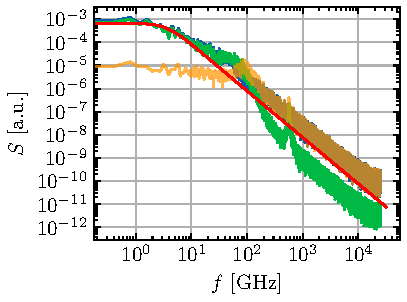
\includegraphics{bilder/plots/Bz_0mT/spectral_power_densities_26.03meV.pdf}}
    \subcaptionbox{Autokorrelation von ursprünglichem, bereinigtem Telegrafenrauschen und Differenz. \label{fig:dominanz-autocorr}}{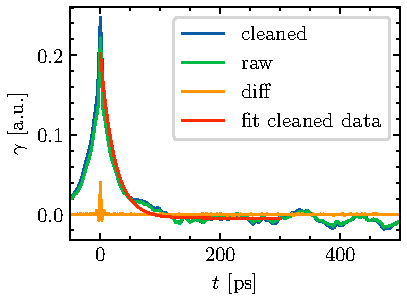
\includegraphics{bilder/plots/Bz_0mT/autocorr_26.03meV.pdf}}
    \caption{Dominanz des Telegrafenrauschen in der Frequenzdomäne. Simulation bei \SI{26.03}{\milli\electronvolt} ohne externes Magnetfeld }\label{fig:dominanz-tgr}
\end{figure}

Beim direkten betrachten des Rauschsignals ist nicht klar erkennbar, ob das statistische oder das Telegrafenrauschen dominiert. Wenn man jedoch die Spektrale Leistungsdichte oder die Autokorrelation bzw. Autocovarianz betrachtet, ist deutlich erkennbar, dass das Telegrafenrauschen hier den größten Beitrag leistet.


\subsection{Variation der Temperatur}

Im Rahmen der Masterarbeit von Julius Schlegel \cite{schlegel-master} wurden bereits Simulationen für verschiedene Temperaturen durchgeführt. Diese Daten wurden für diesen Teil der Analyse verwendet

\subsubsection{In der Zeitdomäne}

\begin{figure}[H]
    \centering
    \subcaptionbox{Temperaturbereich mit sichtbarem Telegrafenrauschen \label{fig:temp-hist-tg}}{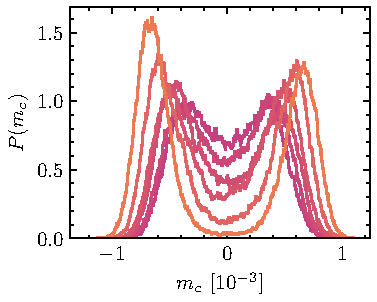
\includegraphics{bilder/plots/temp_comparison_long/mc_hist_tgr.pdf}}
    \subcaptionbox{größerer Temperaturbereich um den Reorientierungsübergang \label{fig:temp-hist-long}}{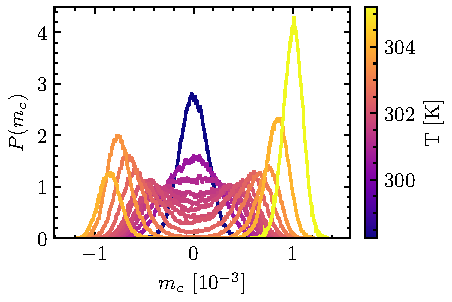
\includegraphics{bilder/plots/temp_comparison_long/mc_hist.pdf}}
    \caption{Wahrscheinlichkeitsdichteverteilung von \(m_c\) für eine Kombination von mehreren Simulationsläufen.}\label{fig:temp-hist}    
\end{figure}

Unterhalb von \SI{300}{\kelvin} existiert nur ein einzelner Zustand, um den \(m_c\) fluktuiert. Je höher die Temperatur wird, desto stärker bilden sich die beiden Zustände aus und das Telegrafenrauschen wird deutlicher sichtbar. Wenn die Temperatur weiter erhöht wird, ist die Mittlere Aufenthaltszeit irgendwann größer als der Simulationszeitraum und kann kein Schaltvorgang mehr beobachtet werden.

Da die Mittlere Aufenthaltszeit ähnlich groß, wie der Simulationszeitraum ist, ist die Wahrscheinlichkeitsdichte der beiden Zustände (in den Simulationsdaten) für hohe Temperaturen hier teilweise unterschiedlich groß. Wenn man mehr und/oder längere Simulationen machen würde, wären die beiden Niveaus für die gelb-orangenen plots in \cref{fig:temp-hist} gleich groß.

Da der Einschwingvorgang mit einem Positiven Startwert (was \(m_c\) angeht beginnt, landet das System bei den Temperaturen oberhalb von \SI{305}{\kelvin} immer im oberen Niveau. und wechselt von dort nicht ins untere Niveau. \todo{testen, ob bei anderem Einschwingvorgang unteres Niveau bevorzugt wird?}

\begin{figure}[H]
    \centering
    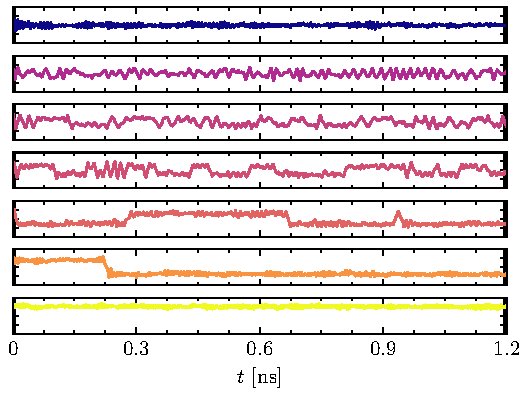
\includegraphics{bilder/plots/temp_comparison_long/mc_time.pdf}
    \caption{\(m_c\) im Zeitlichen Verlauf für verschiedene Temperaturen. Die Daten sind jeweils aus einem einzelnen Simulationslauf. Die Colormap ist hierbei identisch zu der in \cref{fig:temp-hist}. Die y-achse reicht jeweils von \num{-2e-3} bis \num{+2e-3}}\label{fig:temp-time}
\end{figure}

\begin{figure}[H]
    \centering
    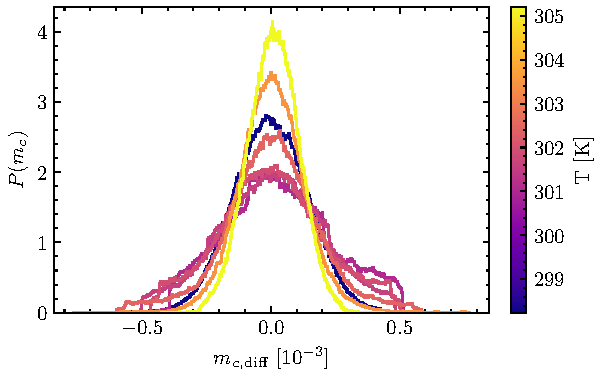
\includegraphics{bilder/plots/temp_comparison_long/mc_diff_hist.pdf}
    \caption{Wahrscheinlichkeitsdichteverteilung für Differenz zwischen rohem Signal und extrahiertem Telegrafenrauschen von \(m_c\) (entspricht extrahiertem statistisches Rauschen)}\label{fig:temp-diff-hist}    
\end{figure}

Wenn vom rohen Signal das Telegrafenrauschen abgezogen wird (oder der Mittelwert, wenn nur ein Zustand existiert), bleibt ein statistisches Rauschen übrig, dessen Histogramm einer Gaußverteilung entspricht \cref{fig:temp-diff-hist}. 

Anhand der Abweichung von einer Gausverteilung im Randbereich (Sprünge statt kontinuierlicher Übergang) sind die Schwellenwerte, die der Algorithmus für die Zustände bestimmt hat, erkennbar.

Diese Verteilung ist für den Temperaturbereich mit aktivem Telegrafenrauschen deutlich breiter, als oberhalb und unterhalb. Dies Liegt wahrscheinlich auch vorallem an den Datenpunkten im Bereich zwischen den zwei Zuständen, welche nicht von der Gausverteilung beschrieben werden (siehe \cref{fig:fit_func_comp}).

Im nachfolgenden Bereich werden meist nurnoch die 6 simulierten Temperaturen mit klar erkennbarem Telegrafenrauschen betrachtet (vgl. \cref{fig:temp-hist-tg}) Daher ändert sich die Farbzuordnung der Temperaturen in den Plots.

\begin{figure}[H]
    \centering
    \subcaptionbox{einzelner Datenpunkt für jede einzelne Simulation \todo{plot relevant?}\label{fig:temp-switch-count-scatter}}{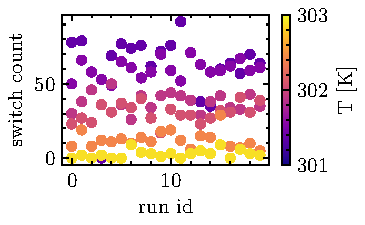
\includegraphics{bilder/plots/temp_comparison/switch_count_scatter.pdf}}
    \subcaptionbox{Mittel-, Extremwerte und Verteilung für jede Simulationstemperatur \label{fig:temp-switch-count-violin}}{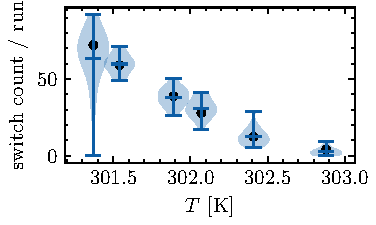
\includegraphics{bilder/plots/temp_comparison/switch_count_violin.pdf}}
    \caption{Temperaturabhängigkeit der Anzahl an Schaltvorgängen \todo{pro welches Zeitinterval?} \todo{über kette berechneten wert in Plot b einfügen}}\label{fig:temp-switch-count}
\end{figure}

Die ansteigende Anzahl an Schaltvorgängen lässt sich auch in \cref{fig:temp-switch-count} gut erkennen. Außerdem sieht man in \cref{fig:temp-switch-count-scatter} einige Simulationsläufe, deren Werte aufgrund der Kurzen Simulationszeit (und daher teilweise das Telegrafenrauschen nicht immer korrekt extrahiert werden konnte) stark von den anderen abweichen.

\begin{figure}[H]
    \centering
    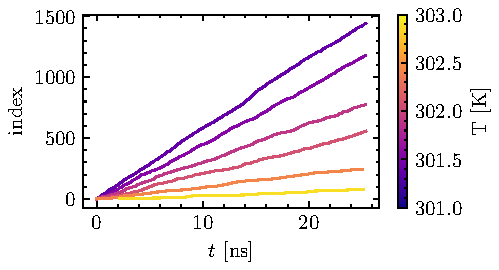
\includegraphics{bilder/plots/temp_comparison/switch_events.pdf}
    \caption{Zeitpunkt an dem ein Schaltvorgang stattfindet \todo{use scatter?}}\label{fig:switch-events}
\end{figure}

In \cref{fig:switch-events} lässt sich gut erkennen, dass die Schaltvorgänge gleichverteilt sind und Aufgrund der hohen Zahl an Schaltvorgängen, die zusätzlichen Schaltvorgänge durch die Verkettung nicht ins Gewicht fallen.

\begin{figure}[H]
    \centering
    \subcaptionbox{einzelner Datenpunkt für jede einzelne Simulation\label{fig:temp-up-percentage-scatter}}{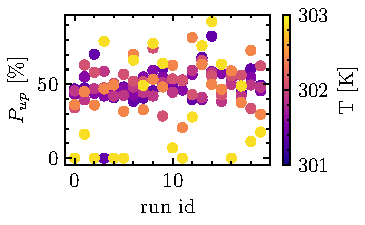
\includegraphics{bilder/plots/temp_comparison/up_percentage_scatter.pdf}}
    \subcaptionbox{Mittel-, Extremwerte und Verteilung für jede Simulationstemperatur \todo{über kette berechneten wert einfügen} \label{fig:temp-up-percentage-violin}}{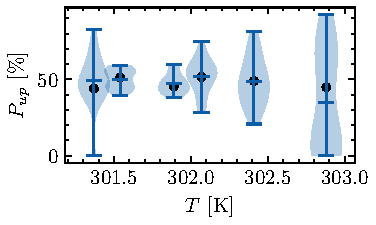
\includegraphics{bilder/plots/temp_comparison/up_percentage_violin.pdf}}
    \caption{Aufenthaltszeit im oberen Zustand}\label{fig:temp-up-percentage}
\end{figure}

Die Aufenthaltswahrscheinlichkeit für beide Zustände liegt in dem Temperaturbereich bei 50\%, aber für die betrachtung der Mittleren Aufenthaltszeit wird die Zahl der Simulationsläufe, in denen sich das System nur in einem Zustand befindet für höhere Temperaturen immer größer.

\subsubsection{In der Frequenzdomäne}

\todo{Erklärrung, warum die Daten in der Zeitdomäne experimentell nicht messbar sind.}

\begin{figure}[H]
    \centering
    \subcaptionbox{aus ursprünglichem Signal \label{fig:temp-spd-source}}{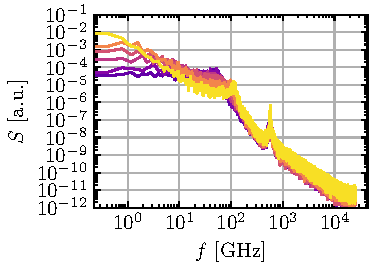
\includegraphics{bilder/plots/temp_comparison/spectral_power_density.pdf}}
    \subcaptionbox{aus bereinigtem Telegrafenrauschen \label{fig:temp-spd-clean}}{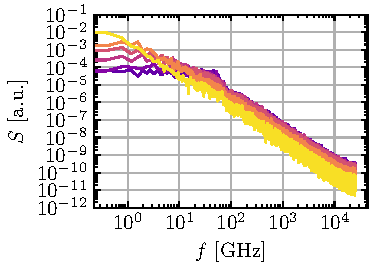
\includegraphics{bilder/plots/temp_comparison/spectral_power_density_cleaned.pdf}}
    \subcaptionbox{aus Differenz, bzw. statistischem Rauschen \label{fig:temp-spd-diff}}{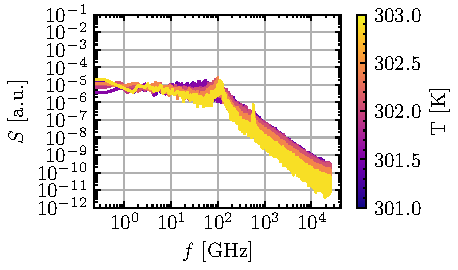
\includegraphics{bilder/plots/temp_comparison/spectral_power_density_diff.pdf}}
    \caption{Spektrale Leistungsdichten für verschiedene Temperaturen \todo{nur eine colorbar}\todo{In Anhang verschieben?}}\label{fig:temp-spd}
\end{figure}


\begin{figure}[H]
    \centering
    \subcaptionbox{aus ursprünglichem Signal \todo{mit fit?}\label{fig:temp-autocorr-source}}{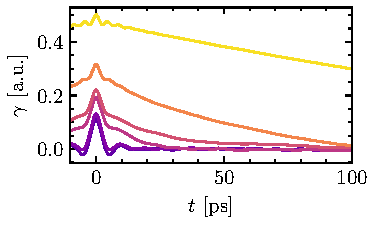
\includegraphics{bilder/plots/temp_comparison/autocorrelation.pdf}}
    \subcaptionbox{aus bereinigtem Telegrafenrauschen \todo{identischer plot?} \todo{fit mit konvergenz gegen 0 statt const.}\label{fig:temp-autocorr-clean}}{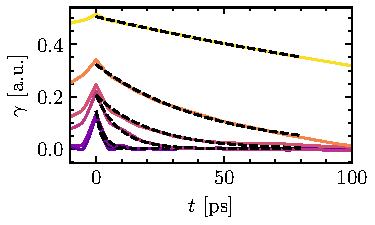
\includegraphics{bilder/plots/temp_comparison/autocorrelation_cleaned.pdf}}
    \subcaptionbox{aus Differenz, bzw. statistischem Rauschen \label{fig:temp-autocorr-diff}}{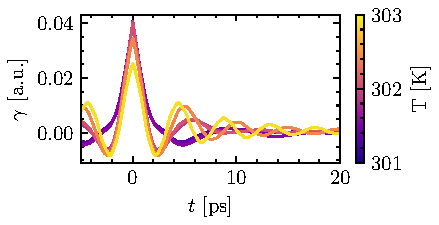
\includegraphics{bilder/plots/temp_comparison/autocorrelation_diff.pdf}}
    \caption{Autokorrelation für verschiedene Temperaturen \todo{nur eine colorbar}}\label{fig:temp-autocorr}
\end{figure}

Da beide Zustände gleich wahrscheinlich sind, Konvergiert die Autokorrelationsfunktion für große Zeiten gegen 0 und ist daher identisch zur Autokovarianz. 

\todo{Berechnung MDT aus Autokorrelation}

Aus Autokorrelationszeit lässt sich die mittlere Aufenthaltszeit mit der Formel \todo{verknüpfung} berechnen.

Aus dem extrahiertem Telegrafenrauschen lassen sich die Aufenthaltszeiten direkt herauslesen. 

\begin{figure}[H]
    \centering
    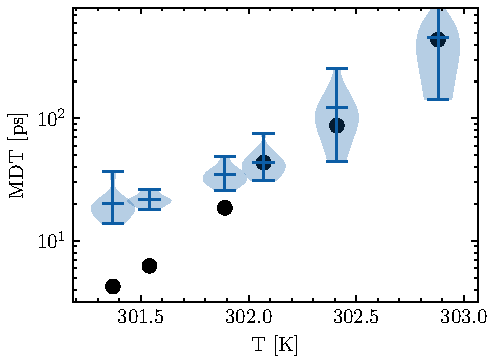
\includegraphics{bilder/plots/temp_comparison/mean_dwell_time_comparison.pdf}
    \caption{Mittlere Aufenthaltszeiten aus Zeitlicher Analyse (Violinenplot) und aus exponentiellem Fit der Autokorrelationsfunktion (schwarze Punkte)}\label{fig:temp-mdt-comp}
\end{figure}

\todo{erklärung für starke abweichung bei niedrigen Temperaturen}
\todo{oder scheint die Abweichung nur so groß?}
\todo{Telegrafenrauschen nichtmehr dominant in Autokovarianz?}
\todo{oder undershoot problem?}

\begin{figure}[H]
    \centering
    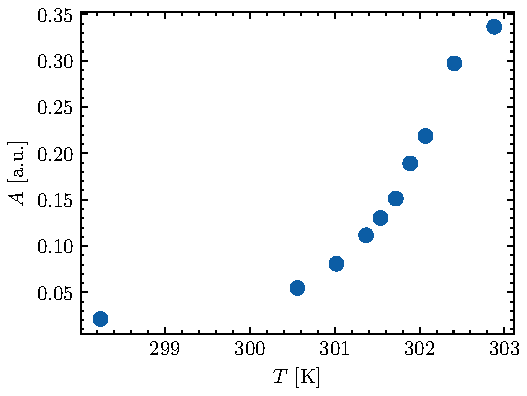
\includegraphics{bilder/plots/temp_comparison_long/rauschamplitude.pdf}
    \caption{Rauschamplitude für verschiedene Temperaturen}\label{fig:temp-autocorr-amplitude}
\end{figure}

Die Amplitude der Autokorrelationsfunktion steigt mit Erhöhung der Temperatur auch immer weiter an.

\subsection{In externem Magnetfeld}

\todo{in plots \(B_z\) statt \(Bz\) nutzen}

\begin{figure}[H]
    \centering
    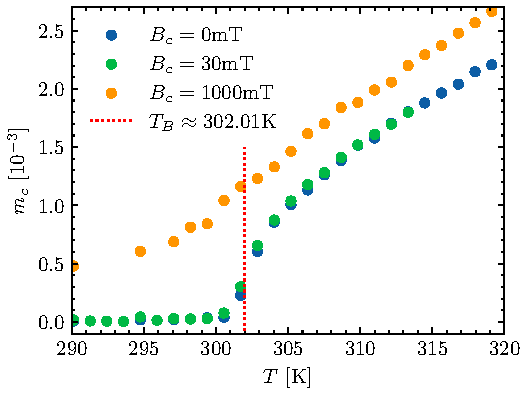
\includegraphics{bilder/plots/Bz_comparison/critical_temperature.pdf}
    \caption{Kritische Temperatur bei schwachem Magnetfeld in z-Richtung}\label{fig:bz-crit-temp}
\end{figure}

\todo{erklärung bei so geringen Magnetfeldern wird der Reorientierungsübergang nicht aufgeweicht}

\begin{figure}[H]
    \centering
    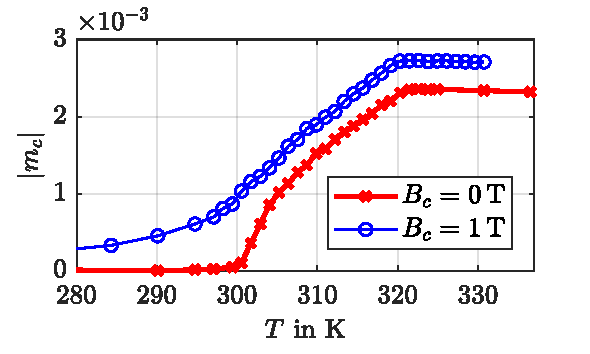
\includegraphics{bilder/jschlege/Magnetization_z.pdf}
    \caption{Kritische Temperatur bei starkem Magnetfeld in z-Richtung \cite{schlegel-master}\todo{selbst neu plotten zusammen mit einer datenreihe aus \cref{fig:bz-crit-temp}}}\label{fig:high-bz-crit-temp}
\end{figure}

\todo{welche bedingungen Bleiben für die nachfolgenden Simulationen gleich?}

Das Magnetfeld wird in z-Richtung angelegt, die c-Richtung im Kristall ist aber identisch zur z-Richtung im externen kartesischen koordinatensystem.

In den Simulationen wird auch immer nur ein konstantes Magnetfeld verwendet.

Als Temperatur wurde für jeden Simulationslauf \( \SI{26.025}{\milli\electronvolt} \approx \SI{302}{\kelvin}\) verwendet.

Der Simulationszeitraum beträgt für alle Simulationsläufe etwa \SI{2.5}{\nano\s}

\begin{figure}[H]
    \centering
    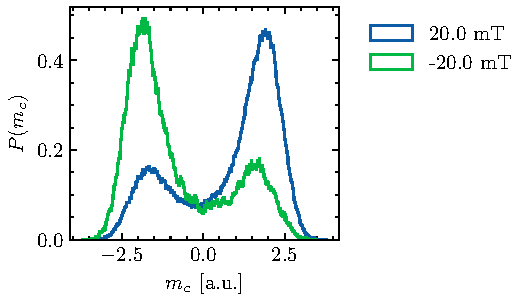
\includegraphics{bilder/plots/Bz_sign_comparison/20mT_hist_comp.pdf}
    \caption{Wahrscheinlichkeitsdichteverteilung von \(m_c\) bei einem externen Magnetfeld von \SI{20}{\milli\tesla} mit entgegengesetzter Richtung}\label{fig:bz-sign-hist}
\end{figure}

Das System scheint sich bei angelegtem B-Feld in entgegengesetzter Richtung Symmetrisch zu verhalten. Dies wurde aber nicht weiter untersucht.


\subsubsection{In der Zeitdomäne}

\begin{figure}[H]
    \centering
    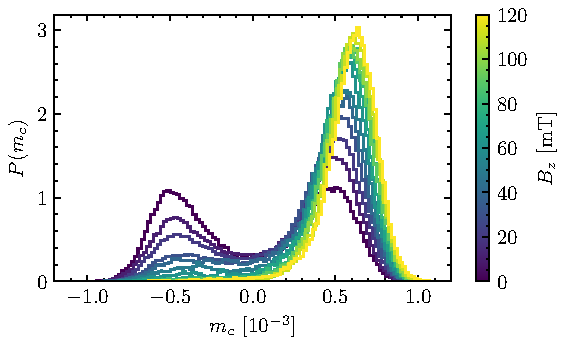
\includegraphics{bilder/plots/max_Bz/mc_hist.pdf}
    \caption{Wahrscheinlichkeitsdichteverteilung von \(m_c\) für eine Kombination von mehreren Simulationsläufen und bei verschieden starken externen Magnetfeldern}\label{fig:b-hist}    
\end{figure}

Anders als bei der Variation der Temperatur ohne externes Magnetfeld (\cref{fig:temp-hist}), sind die beiden Zustände nicht mehr Gleichverteilt. Wenn einer der beiden Peaks zu klein wird, kann der Algorithmus das Telegrafenrauschen nicht mehr extrahieren. 

Da das obere Niveau jetzt aber eine deutlich höhere Aufenthaltswahrscheinlichkeit hat, kommt es auch (je nach stärke des B-Feldes) zu deutlich weniger zusätzlichen Schaltvorgängen bei der Verkettung mehrerer Simulationsläufe.

\todo{erklärung verschiebung der Niveau peaks}

\todo{was passiert in den anderen Komponenten von m?}

\begin{figure}[H]
    \centering
    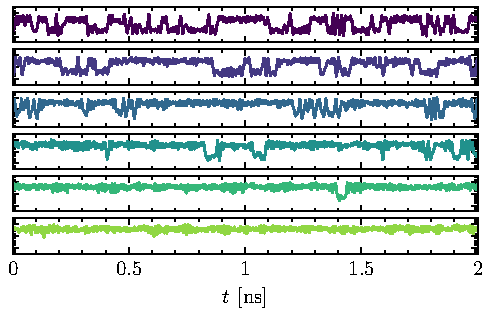
\includegraphics{bilder/plots/max_Bz/mc_time.pdf}
    \caption{Ausschnitt von \(m_c\) im Zeitlichen Verlauf bei verschieden starken externen Magnetfeldern . Die Colormap ist hier identisch zu der von \cref{fig:b-hist}. Die y-Achse reicht hier jeweils von \num{-1.5e-3} bis \num{+1.5e-3}}\label{fig:b-time}    
\end{figure}

\begin{figure}[H]
    \centering
    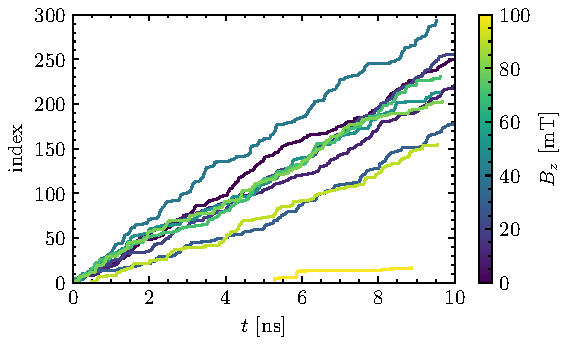
\includegraphics{bilder/plots/max_Bz/switch_events.pdf}
    \caption{Zeitpunkt an dem ein Schaltvorgang stattfindet}\label{fig:bz-switch-events}   
\end{figure}

\todo{hier bei 100mT garantiert kein problem aufgrund der Verkettung, da sich das system quasi durchgängig im oberen Niveau befindet}

In Manchen Simulationsläufen bei \SI{100}{\milli\tesla} findet gar kein Schaltvorgang statt.

\begin{figure}[H]
    \centering
    \subcaptionbox{Aufenthaltszeit im oberen Zustand. Bestimmt über einzelne Simulationsläufe (Violinplot) und über Kette mehrerer Simulationen (schwarze Punkte) \label{fig:bz-up-percentage-violin}}{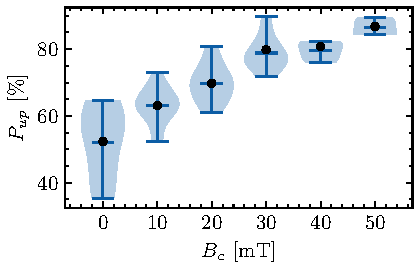
\includegraphics{bilder/plots/max_Bz/up_percentage_violin.pdf}}
    \subcaptionbox{Mittlere Aufenthaltszeit in oberem (blau) und unterem (grün) Zustand in Prozent. Die wagrechte Linie kennzeichnet hierbei den Mittelwert und der Violinplot die Verteilung der verschiedenen Aufenthaltszeiten auf dem jeweiligen Niveau \label{fig:bz-state-times-comp}}{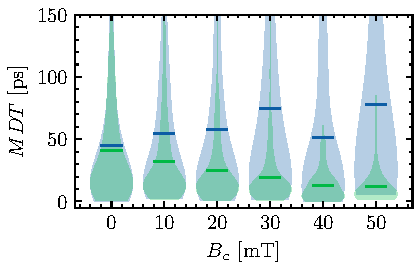
\includegraphics{bilder/plots/max_Bz/state_times_comp.pdf}}
    \caption{Abhängigkeit der Aufenthaltszeit von der Magnetfeldstärke}\label{fig:bz-state-times}
\end{figure}

\todo{mittlere Aufenthaltszeit (nicht aufgeteilt nach up/down)}

\begin{figure}[H]
    \centering
    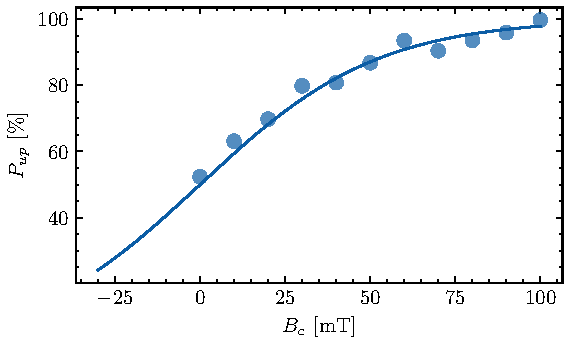
\includegraphics{bilder/plots/max_Bz/up_percentage_fit.pdf}
    \caption{Die Aufenthaltszeit im oberen Zustand mit einer Sigmoid-Funktion gefittet. Die Datenpunkte wurden dabei mittels des Algorithmus aus mehreren verketteten Simulationsläufen extrahiert}\label{fig:bz-up-percentage}
\end{figure}

\todo{fitparameter obere schranke diskutieren}

\todo{worin ist das sonst erkennbar, dass kein Schaltvorgang mehr stattfindet?}

\subsubsection{In der Frequenzdomäne}


\begin{figure}[H]
    \centering
    \subcaptionbox{aus ursprünglichem Signal\label{fig:bz-spd-source}}{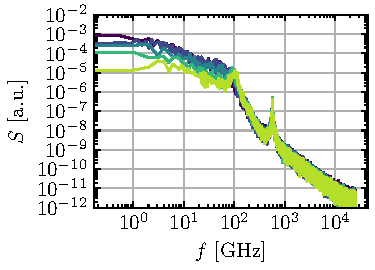
\includegraphics{bilder/plots/max_Bz/spectral_power_density.pdf}}
    \subcaptionbox{aus bereinigtem Telegrafenrauschen\label{fig:bz-spd-clean}}{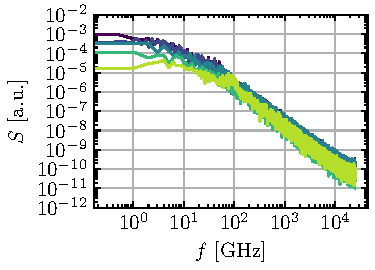
\includegraphics{bilder/plots/max_Bz/spectral_power_density_cleaned.pdf}}
    \subcaptionbox{aus Differenz, bzw. statistischem Rauschen \label{fig:bz-spd-diff}}{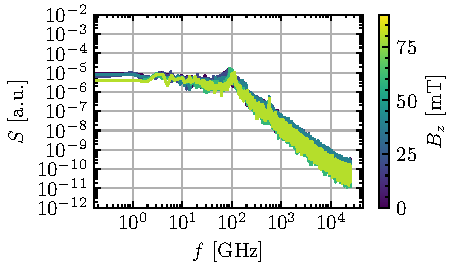
\includegraphics{bilder/plots/max_Bz/spectral_power_density_diff.pdf}}
    \caption{Spektrale Leistungsdichten bei verschiedenen Magnetfeldstärken}\label{fig:bz-spd}
\end{figure}


\begin{figure}[H]
    \centering
    \subcaptionbox{aus ursprünglichem Signal \label{fig:bz-autocorr-source}}{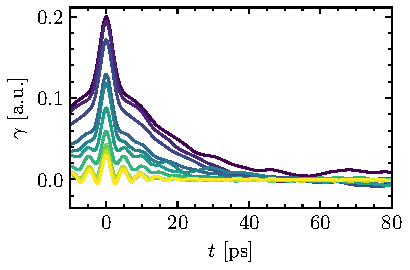
\includegraphics{bilder/plots/max_Bz/autocov.pdf}}
    \subcaptionbox{aus bereinigtem Telegrafenrauschen \todo{ohne fit und nur bis 75ps}\label{fig:bz-autocorr-clean}}{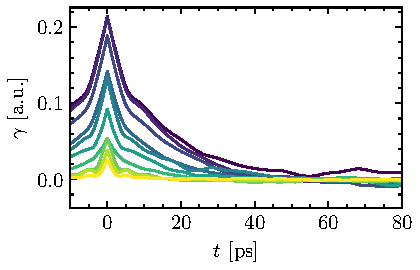
\includegraphics{bilder/plots/max_Bz/autocov_cleaned.pdf}}
    \subcaptionbox{aus Differenz, bzw. statistischem Rauschen \label{fig:bz-autocorr-diff}}{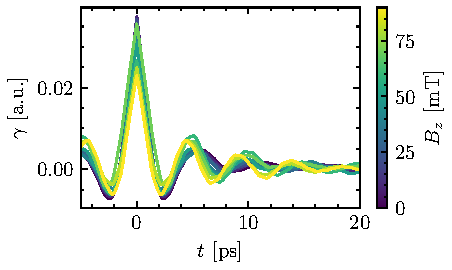
\includegraphics{bilder/plots/max_Bz/autocorrelation_diff.pdf}}
    \caption{Autokovarianz für verschiedene Magnetfeldstärken \todo{nur eine colorbar. plots etwas größer}}\label{fig:bz-autocov}
\end{figure}

\todo{Autokorrelation vs Autokovarianz}


\todo{Die Mean Dwell time ist nicht aus der Autokorrelation Bestimmbar (Mittlere Mean Dwell time)}


\begin{figure}[H]
    \centering
    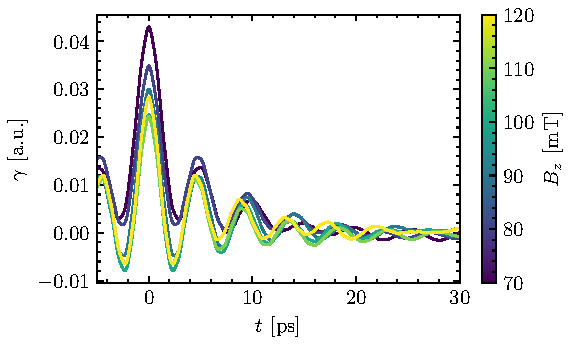
\includegraphics{bilder/plots/max_Bz/autocov_high.pdf}
    \caption{Autokovarianz für hohe Magnetfeldstärken}\label{fig:bz-autocov-high}
\end{figure})

\todo{erkennbar, dass kein telegrafenraushcen mehr stattfindet}

\begin{figure}[H]
    \centering
    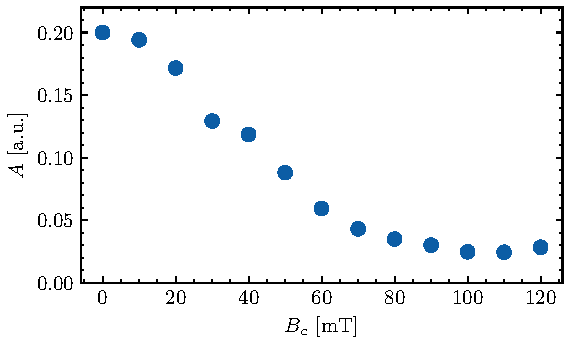
\includegraphics{bilder/plots/max_Bz/rauschamplitude.pdf}
    \caption{Amplitude der Autokovarianz abhängig von \(B_z\)}\label{fig:bz-rauschampl}
\end{figure}

Die Amplitude der Autokovarianz wird bei Erhöhung der Temperatur immer kleiner und oberhalb von \SI{100}{\milli\tesla} minimal. Sie scheint danach wieder anzusteigen, Die Abweichung des Datenpunktes bei \SI{120}{\milli\tesla} ist aber alleine nicht aussagekräftig. 

\todo{warum fällt die Rauschamplitude ab?}

% bibliography (temporary)
% \bibliography{literatur} \todo{comment out before compiling main.tex}

\end{document}